\section{Reachable Set Analysis}

\begin{figure}
	\centering
	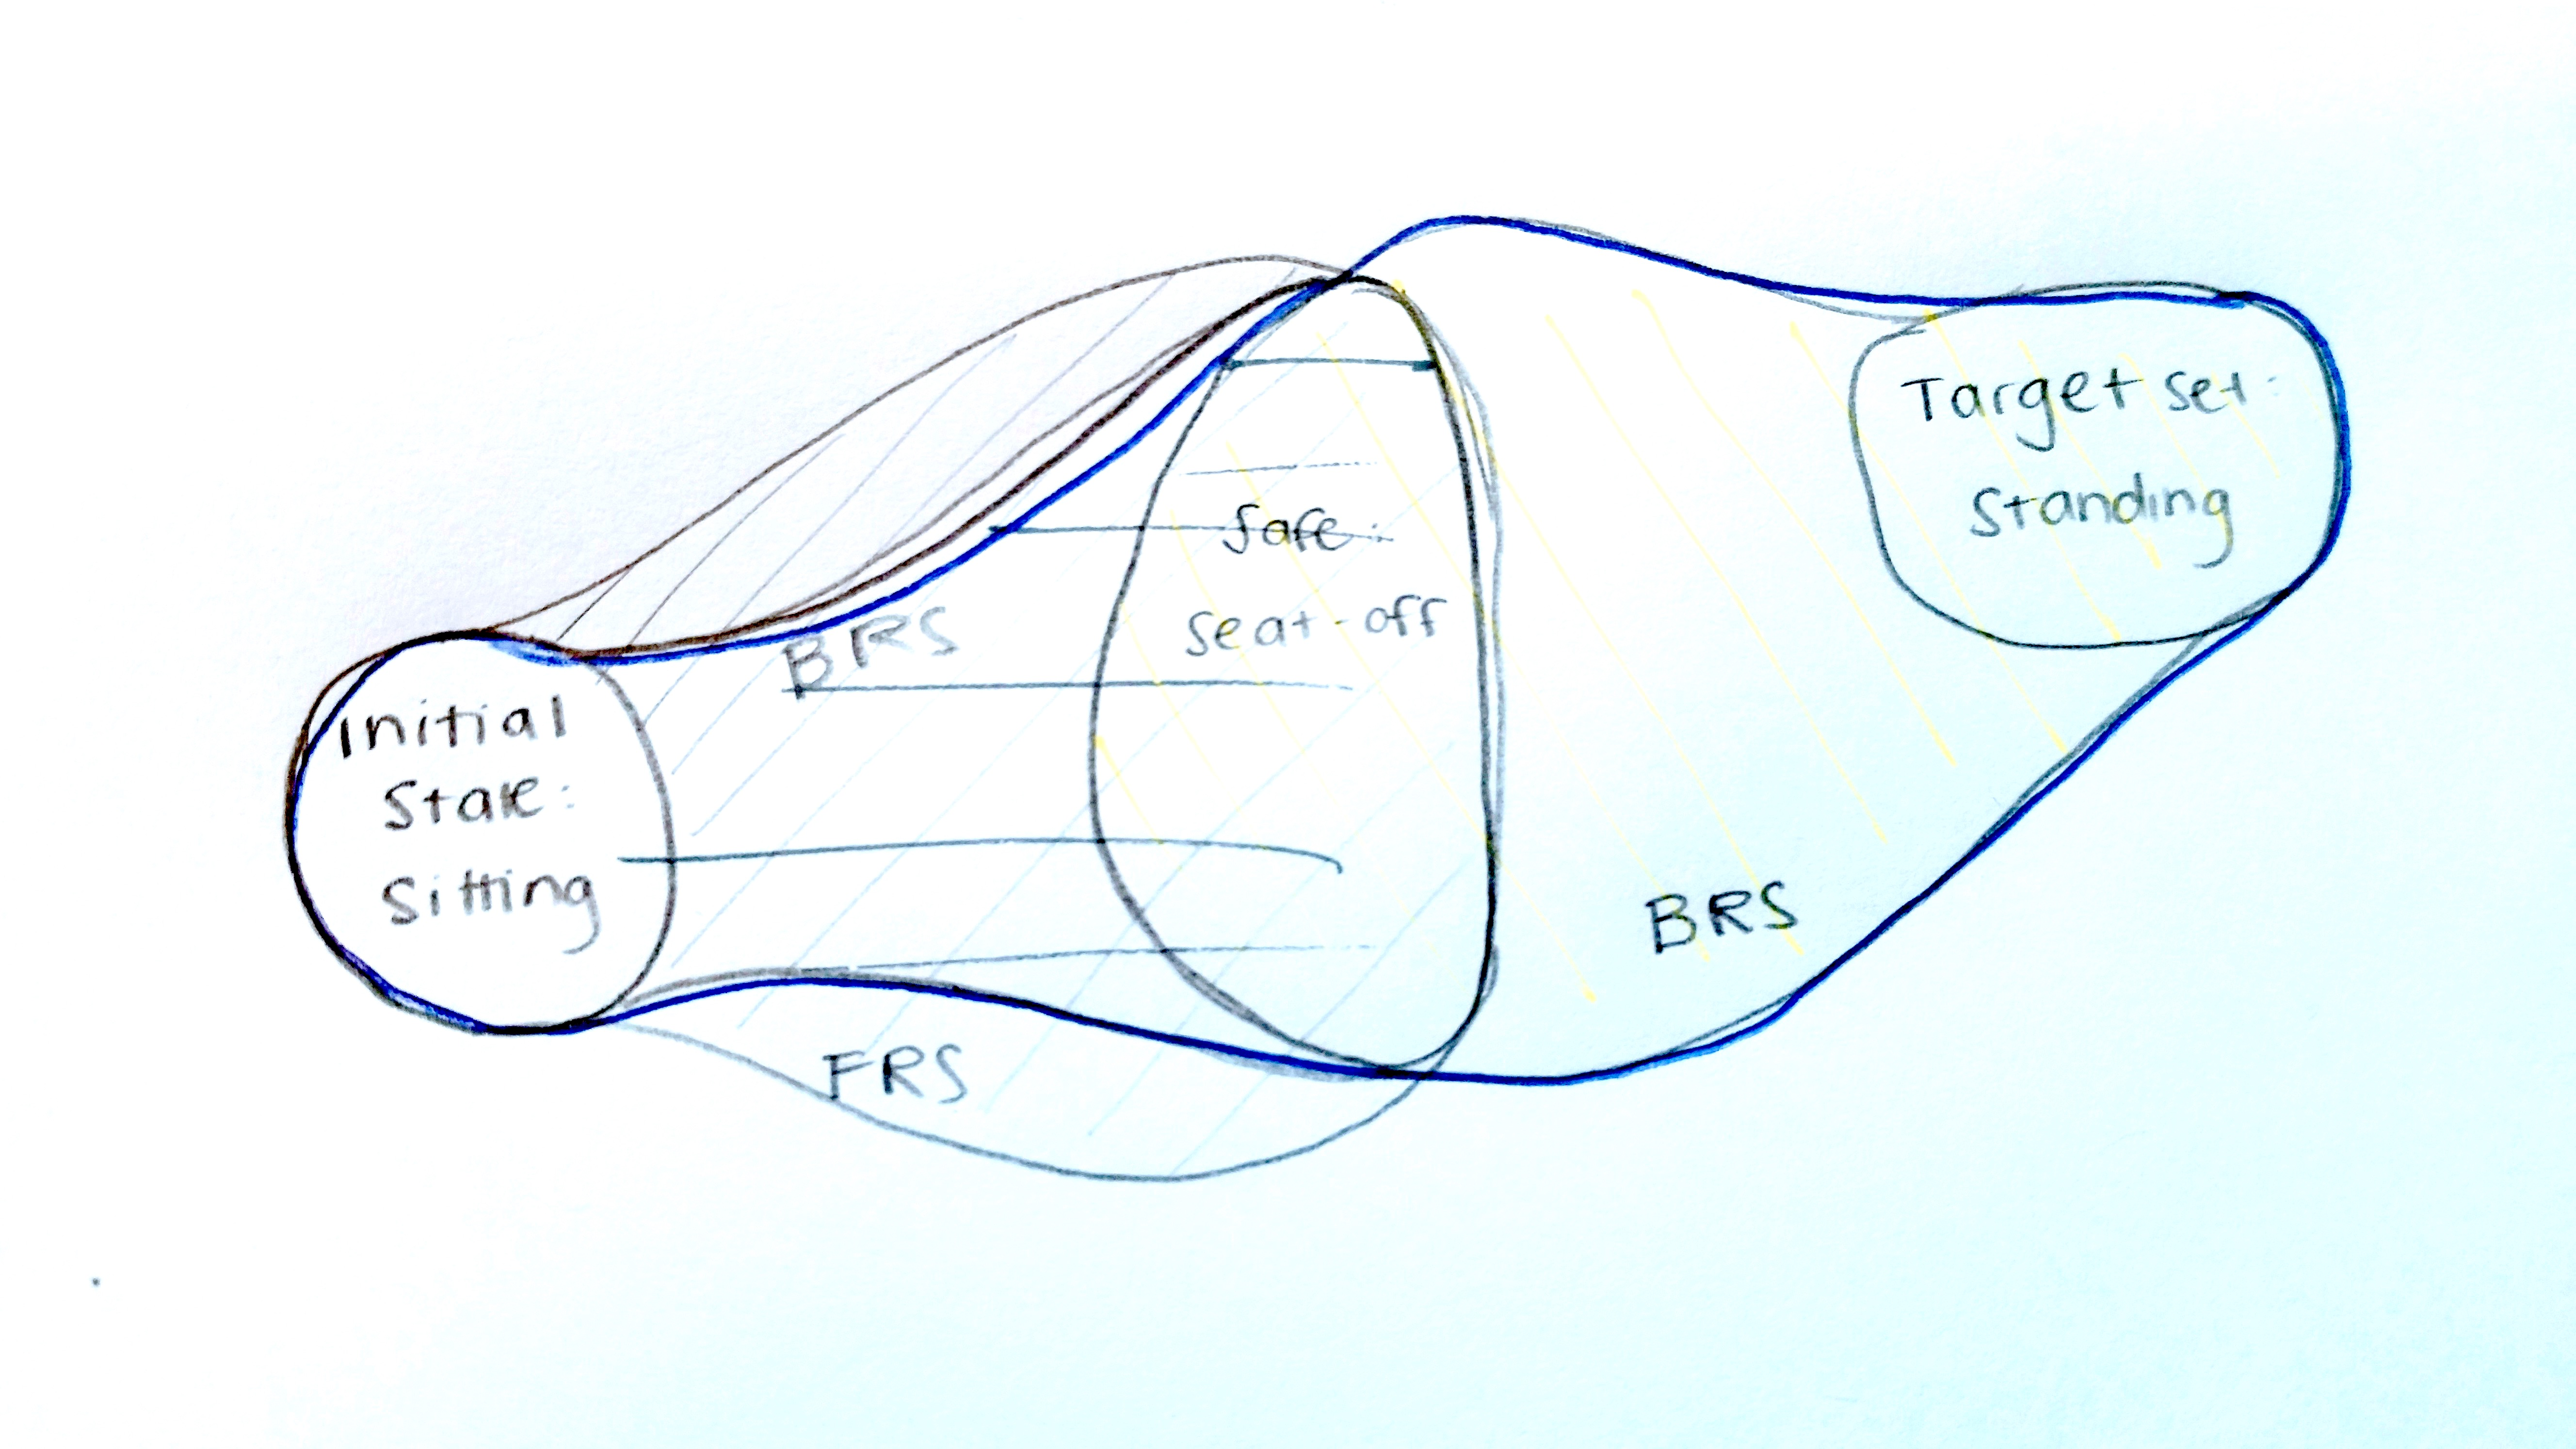
\includegraphics[width=3.5in]{figures/reachableSets.jpg}
	\caption{Reachable sets for STS motion.}
	\label{fig:hybrid}
\end{figure}

[Basic explanation of how HJ reachability analysis works]

We specify initial and final conditions on the states. The target set, representing the standing goal, is defined by a range of knee and hip angles near vertical with near-zero angular velocities. The initial seated condition is defined by a vertical HAT with zero-velocity. We compute a forwards reachable set, computing the set of states that be reached along trajectories which originate in the initial, seated position.

Separately, we compute a backwards reachable set, specifying conditions on the joint states which define the target set. The backwards reachable set represents the set of initial conditions of trajectories which enter the desired target set. In the case of sit-to-stand the backwards reachable set denotes the joint angles and velocities from which it is possible to reach a standing position. 

The intersection of the forwards and backwards reachable sets represent the states for which it is safe to transition between the seated and rising modes. From this final state, we compute a backwards reachable set to determine the allowable mode 1 states.